%% BioMed_Central_Tex_Template_v1.06
%%                                      %
%  bmc_article.tex            ver: 1.06 %
%                                       %

%%IMPORTANT: do not delete the first line of this template
%%It must be present to enable the BMC Submission system to
%%recognise this template!!

%%%%%%%%%%%%%%%%%%%%%%%%%%%%%%%%%%%%%%%%%
%%                                     %%
%%  LaTeX template for BioMed Central  %%
%%     journal article submissions     %%
%%                                     %%
%%          <8 June 2012>              %%
%%                                     %%
%%                                     %%
%%%%%%%%%%%%%%%%%%%%%%%%%%%%%%%%%%%%%%%%%


%%%%%%%%%%%%%%%%%%%%%%%%%%%%%%%%%%%%%%%%%%%%%%%%%%%%%%%%%%%%%%%%%%%%%
%%                                                                 %%
%% For instructions on how to fill out this Tex template           %%
%% document please refer to Readme.html and the instructions for   %%
%% authors page on the biomed central website                      %%
%% http://www.biomedcentral.com/info/authors/                      %%
%%                                                                 %%
%% Please do not use \input{...} to include other tex files.       %%
%% Submit your LaTeX manuscript as one .tex document.              %%
%%                                                                 %%
%% All additional figures and files should be attached             %%
%% separately and not embedded in the \TeX\ document itself.       %%
%%                                                                 %%
%% BioMed Central currently use the MikTex distribution of         %%
%% TeX for Windows) of TeX and LaTeX.  This is available from      %%
%% http://www.miktex.org                                           %%
%%                                                                 %%
%%%%%%%%%%%%%%%%%%%%%%%%%%%%%%%%%%%%%%%%%%%%%%%%%%%%%%%%%%%%%%%%%%%%%

%%% additional documentclass options:
%  [doublespacing]
%  [linenumbers]   - put the line numbers on margins

%%% loading packages, author definitions

\documentclass[twocolumn]{bmcart}% uncomment this for twocolumn layout and comment line below
%\documentclass{bmcart}

%%% Load packages
\usepackage{amsthm,amsmath}
\usepackage{siunitx}
\usepackage{mfirstuc}
%\RequirePackage{natbib}
\usepackage[colorinlistoftodos]{todonotes}
\RequirePackage{hyperref}
\usepackage[utf8]{inputenc} %unicode support
%\usepackage[applemac]{inputenc} %applemac support if unicode package fails
%\usepackage[latin1]{inputenc} %UNIX support if unicode package fails
\usepackage[htt]{hyphenat}

\usepackage{array}
\newcolumntype{L}[1]{>{\raggedright\let\newline\\\arraybackslash\hspace{0pt}}p{#1}}

%%%%%%%%%%%%%%%%%%%%%%%%%%%%%%%%%%%%%%%%%%%%%%%%%
%%                                             %%
%%  If you wish to display your graphics for   %%
%%  your own use using includegraphic or       %%
%%  includegraphics, then comment out the      %%
%%  following two lines of code.               %%
%%  NB: These line *must* be included when     %%
%%  submitting to BMC.                         %%
%%  All figure files must be submitted as      %%
%%  separate graphics through the BMC          %%
%%  submission process, not included in the    %%
%%  submitted article.                         %%
%%                                             %%
%%%%%%%%%%%%%%%%%%%%%%%%%%%%%%%%%%%%%%%%%%%%%%%%%


%\def\includegraphic{}
%\def\includegraphics{}

%%% Put your definitions there:
\startlocaldefs
\endlocaldefs


%%% Begin ...
\begin{document}

%%% Start of article front matter
\begin{frontmatter}

\begin{fmbox}
\dochead{Report from 2015 Brainhack Americas (MX)}

%%%%%%%%%%%%%%%%%%%%%%%%%%%%%%%%%%%%%%%%%%%%%%
%%                                          %%
%% Enter the title of your article here     %%
%%                                          %%
%%%%%%%%%%%%%%%%%%%%%%%%%%%%%%%%%%%%%%%%%%%%%%

\title{The Neuroimaging Data Model (NIDM) API}
\vskip2ex
\projectURL{Project URL: \url{http://nidm-api.readthedocs.org}}

\author[
addressref={aff1},
corref={aff1},
email={vsochat@stanford.edu}
]{\inits{VS} \fnm{Vanessa} \snm{Sochat}}
\author[
addressref={aff2,aff3},
%
email={nolan.nichols@gmail.com}
]{\inits{NN} \fnm{Nolan} \snm{Nichols}}

%%%%%%%%%%%%%%%%%%%%%%%%%%%%%%%%%%%%%%%%%%%%%%
%%                                          %%
%% Enter the authors' addresses here        %%
%%                                          %%
%% Repeat \address commands as much as      %%
%% required.                                %%
%%                                          %%
%%%%%%%%%%%%%%%%%%%%%%%%%%%%%%%%%%%%%%%%%%%%%%

\address[id=aff1]{%
  \orgname{Program in Biomedical Informatics, Stanford University},
  \city{Stanford},
  \street{1265 Welch Road},
  \postcode{94306},
  \postcode{California},
  \cny{USA}
}
\address[id=aff2]{%
  \orgname{SRI International},
  \city{Menlo Park},
  \street{333 Ravenswood Ave},
  \postcode{94025},
  \postcode{California},
  \cny{USA}
}
\address[id=aff3]{%
  \orgname{Department of Psychiatry and Behavioral Sciences, Stanford University},
  \city{Stanford},
  \street{1265 Welch Road},
  \postcode{94306},
  \postcode{California},
  \cny{USA}
}

%%%%%%%%%%%%%%%%%%%%%%%%%%%%%%%%%%%%%%%%%%%%%%
%%                                          %%
%% Enter short notes here                   %%
%%                                          %%
%% Short notes will be after addresses      %%
%% on first page.                           %%
%%                                          %%
%%%%%%%%%%%%%%%%%%%%%%%%%%%%%%%%%%%%%%%%%%%%%%

\begin{artnotes}
\end{artnotes}

%\end{fmbox}% comment this for two column layout

%%%%%%%%%%%%%%%%%%%%%%%%%%%%%%%%%%%%%%%%%%%%%%
%%                                          %%
%% The Abstract begins here                 %%
%%                                          %%
%% Please refer to the Instructions for     %%
%% authors on http://www.biomedcentral.com  %%
%% and include the section headings         %%
%% accordingly for your article type.       %%
%%                                          %%
%%%%%%%%%%%%%%%%%%%%%%%%%%%%%%%%%%%%%%%%%%%%%%

%\begin{abstractbox}

%\begin{abstract} % abstract
	
%Blank Abstract

%\end{abstract}



%%%%%%%%%%%%%%%%%%%%%%%%%%%%%%%%%%%%%%%%%%%%%%
%%                                          %%
%% The keywords begin here                  %%
%%                                          %%
%% Put each keyword in separate \kwd{}.     %%
%%                                          %%
%%%%%%%%%%%%%%%%%%%%%%%%%%%%%%%%%%%%%%%%%%%%%%

%\vskip1ex

%\projectURL{\url{http://github.com/ccraddock/afni}}
%\projectURL{http://github.com/ccraddock/afni}

% MSC classifications codes, if any
%\begin{keyword}[class=AMS]
%\kwd[Primary ]{}
%\kwd{}
%\kwd[; secondary ]
%\end{keyword}

%\end{abstractbox}
%
\end{fmbox}% uncomment this for twcolumn layout

\end{frontmatter}

%{\sffamily\bfseries\fontsize{10}{12}\selectfont Project URL: \url{http://github.com/ccraddock/afni}}

%%% Import the body from pandoc formatted text
\section{Introduction}\label{introduction}
The sharing of brain research can be aided by the Neuroimaging Data Model (NIDM)[KEATOR TOWARDS STRUCTURED SHARING] \cite{noauthor_undated-jz} \cite{noauthor_undated-pr}. NIDM provides a community-based framework for developing data exchange standards that describe the primary observations, computational workflows, and derived results of neuroimaging studies \cite{noauthor_undated-jv}. While work is underway to integrate NIDM into the software used by the human brain mapping community, only low-level tools are currently available to access and query NIDM documents that rely on a graph-based representation called the Resource Description Framework (RDF) \cite{noauthor_undated-hj}. Further, technologies like RDF and the corresponding query language, SPARQL \cite{noauthor_undated-cp}, pose a steep learning curve for users of standard Web development workflows. With the recent migration of tools for neuroimaging meta analysis \cite{Yarkoni2011-rg}, sharing [CITE Papers from Recent Neuroimage Issue] \cite{Gorgolewski2015-sf}, and visualization [CITE galant, XTK, BrainBrowser, etc]\cite{noauthor_undated-ca} into the Web browser, Web developers will be incentivized by the ability to easily integrate brain data into Web applications using familiar languages and formats. The formats of choice for web development tend to be JavaScript and JavaScript Object Notation (JSON) \cite{Wikipedia_contributors2015-on} \cite{noauthor_undated-tz}, commonly provided by way of an Application Programming Interface (API). The goal of this Brainhack project was to develop infrastructure to serve NIDM documents and queries using an API with a syntax that allows for the easy development of Web-based tools for the neuroimaging community.

\section{Approach}\label{approach}
The \texttt{nidm-api} \cite{noauthor_undated-hq} is a RESTful API and Web application that provides a simplified view of NIDM documents using formats that are accessible to Web developers and researchers without expertise in Linked Open Data (LOD) technologies. It includes two components. First, the \href{https://github.com/incf-nidash/nidm-api}{\texttt{nidm-api}}, is a Python-based executable that works both as a command-line tool to run queries over NIDM documents, as well as to serve a RESTful API to allow a local or cloud-based server to execute queries on documents accessible by URL. Second, \href{https://github.com/incf-nidash/nidm-queries}{\texttt{nidm-queries}} is a repository of SPARQL queries that the \texttt{nidm-api} application dynamically downloads, validates, and serves upon starting the application. This strategy means that NIDM developers can collaboratively construct SPARQL queries without requiring Web developers to gain expertise in LOD technology. The \texttt{nidm-api}, along with serving the queries, also provides a graphical Web interfaces to contribute new queries to the shared repository. By way of being a Python Flask \cite{noauthor_undated-ia} application, this makes the application able to perform as both an executable to serve the API \cite{noauthor_undated-ii}, along with a set of functions that can be integrated into other Python-based frameworks \cite{noauthor_undated-ej} or cloud platforms that provide Python accessibility \cite{noauthor_undated-jw}\cite{Google_undated-aj}. 

\section{Results}\label{results}
\subparagraph{\texorpdfstring{\texttt{Using the API}:}{:}}\label{section}
Installation produces an executable, “nidm” that when run, downloads, validates, and provides a summary of available queries in the \texttt{nidm-queries} repository. A query can be further investigated by selecting its unique identifier: \newline

\textbf{http://localhost:8088/api/7950f524-90e8-4d54-ad6d-7b22af2e895d}\newline

and can then be executed in a RESTful fashion by including a variable to point to a local path or URL of a NIDM document:\newline

\textbf{http://localhost:8088/api/query/7950f524-90e8-4d54-ad6d-7b22af2e895d?ttl=/home/nidm.ttl}\newline

The API then runs the query over the document, and returns the result to the user in JSON.

The same functionality can be achieved on the command line \href{http://nidm-api.readthedocs.org/en/latest/getting-started.html#integration-into-python}{command line} in the case that it is desired to integrate it directly into a server-based Python application.\newline

\subparagraph{\texorpdfstring{\texttt{Generating new queries}:}{:}}\label{section}
Researchers familiar with LOD can run the application in the same fashion, and go to a URL in their local browser (http://localhost:8088/query/new) to reveal \href{http://nidm-api.readthedocs.org/en/latest/development.html#web-query-generator}{an interface} to generate new queries. The web interface asks for a set of \href{http://nidm-api.readthedocs.org/en/latest/development.html#fields}{variables} that are necessary for the \texttt{nidm-api} to serve the query. The query can be previewed, and then downloaded as a JSON object that can be submit to the \texttt{nidm-queries} repository to be added to the application.\newline

\subparagraph{\texorpdfstring{\texttt{Applications using NIDM}:}{:}}\label{section}
As an example of the utility of the NIDM standard, the NIDM results object model \cite{noauthor_undated-if} has recently been integrated into the \href{http://www.neurovault.org}{NeuroVault} database, meaning that neuroimaging researchers can export results pertaining to statistical brain maps from common software \cite{Jenkinson2012-pr} into NeuroVault. An \href{https://github.com/vsoch/nidmviewer}{nidm-viewer} that runs queries over the nidm-results can then parse the coordinates and statistical parameters associated with significant locations of activations to be rendered in a table alongside a visualization of the brain map itself (Figure \ref{fig:01} and \href{http://neurovault.org/collections/877/fsl_course_av.nidm}{example}). The raw data and parameters of the analysis are thus immediately available for sharing and publication, programatically accessible, and viewed from any web browser. 

\begin{figure}[h!]
\begin{center}
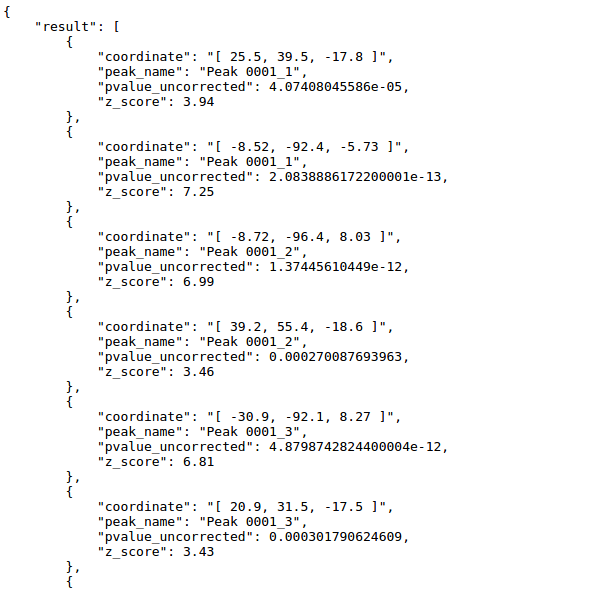
\includegraphics[width=7cm]{img/figure1}
\end{center}
 \textbf{\refstepcounter{figure}\label{fig:01}Figure \arabic{figure}.}{The nidm-viewer in the NeuroVault database queries nidm-result objects to generate an interactive table and statistical brain map.}
\end{figure}

\section{Conclusions}\label{conclusions}

By separating queries from the software to serve them, development of both can be optimized, and the NIDM standard more easily deployed into tools to empower neuroimaging researchers to explore and synthesize results, workflows, and experiments. This application will be further developed to return more modern and desired outputs such as images and interactive graphs \cite{noauthor_undated-fs}, and as the NIDM experiment, workflows, and results standards are further developed. The software and queries are both \href{https://github.com/incf-nidash}{publicly available} and open to contributions.

%%%%%%%%%%%%%%%%%%%%%%%%%%%%%%%%%%%%%%%%%%%%%%
%%                                          %%
%% Backmatter begins here                   %%
%%                                          %%
%%%%%%%%%%%%%%%%%%%%%%%%%%%%%%%%%%%%%%%%%%%%%%

\begin{backmatter}

\section*{Availability of Supporting Data}
More information about this project can be found at: \url{http://nidm-api.readthedocs.org}. Further data and files supporting this project are hosted in the \emph{INCF NIDASH} repositories https://github.com/incf-nidash/nidm-api and https://github.com/incf-nidash/nidm-queries.

\section*{Competing interests}
None

\section*{Author's contributions}
VS and NN wrote the software and wrote the report.

\section*{Acknowledgements}
The authors would like to thank the INCF Neuroimaging Data Sharing Task Force, along with organizers and attendees of Brainhack MX. VS is supported by a William R. Hewlett Stanford Graduate Fellowship and a National Science Foundation Fellowship. NN is supported by NIH NIAAA and OD (NCANDA Data Analysis Component, NIH 1 U01 AA021697; BD2K Supplement, NIH 1 U01 AA021697-04S1).
  
%%%%%%%%%%%%%%%%%%%%%%%%%%%%%%%%%%%%%%%%%%%%%%%%%%%%%%%%%%%%%
%%                  The Bibliography                       %%
%%                                                         %%
%%  Bmc_mathpys.bst  will be used to                       %%
%%  create a .BBL file for submission.                     %%
%%  After submission of the .TEX file,                     %%
%%  you will be prompted to submit your .BBL file.         %%
%%                                                         %%
%%                                                         %%
%%  Note that the displayed Bibliography will not          %%
%%  necessarily be rendered by Latex exactly as specified  %%
%%  in the online Instructions for Authors.                %%
%%                                                         %%
%%%%%%%%%%%%%%%%%%%%%%%%%%%%%%%%%%%%%%%%%%%%%%%%%%%%%%%%%%%%%

% if your bibliography is in bibtex format, use those commands:
\bibliographystyle{bmc-mathphys} % Style BST file
\bibliography{brainhack-report} % Bibliography file (usually '*.bib' )

\end{backmatter}
\end{document}